\documentclass{article}
%\documentclass[a4paper,landscape]{article}

\usepackage{graphicx}
\usepackage{tabularx}
\usepackage{adjustbox}
\usepackage{amsmath}
\usepackage{amsfonts}
\usepackage{multirow}

%% Key definitions for text elements. USE THEM
\def\secref#1{Sec.~\ref{#1}}
\def\figref#1{Fig.~\ref{#1}}
\def\tabref#1{Tab.~\ref{#1}}
\def\eqref#1{Eq.~(\ref{#1})}
\def\algref#1{Alg.~\ref{#1}}
\def\appref#1{App.~\ref{#1}}

\newcommand\etal{\emph{et al.}}

\usepackage{rotating}

\usepackage{amsopn}


\newcommand{\bJidx}[1]{\ensuremath{\mathbf{J}^{[#1]}}}
\newcommand{\cose}{\mathrm{cose}}
\newcommand{\bzidx}[1]{\mathbf{z}^{[{#1}]}}
\newcommand{\bxidx}[1]{\mathbf{x}^{[{#1}]}}
\newcommand{\bhidx}[1]{\mathbf{h}^{[{#1}]}}
\newcommand{\bOmegaidx}[1]{\mathbf{\Omega}^{[{#1}]}}
\newcommand{\bSigmaidx}[1]{\mathbf{\Sigma}^{[{#1}]}}
\newcommand{\bHidx}[1]{\mathbf{H}^{[{#1}]}}

\newcommand{\bv}{\mathbf{v}}
\newcommand{\bl}{\mathbf{l}}
\newcommand{\bt}{\mathbf{t}}
\newcommand{\bo}{\mathbf{o}}
\newcommand{\bM}{\mathbf{M}}
\newcommand{\bL}{\mathbf{L}}
\newcommand{\bA}{\mathbf{A}}
\newcommand{\bB}{\mathbf{B}}
\newcommand{\bE}{\mathbf{E}}
\newcommand{\bK}{\mathbf{K}}
\newcommand{\bC}{\mathbf{C}}
\newcommand{\bH}{\mathbf{H}}
\newcommand{\bI}{\mathbf{I}}
\newcommand{\bP}{\mathbf{P}}
\newcommand{\bX}{\mathbf{X}}
\newcommand{\bZ}{\mathbf{Z}}
\newcommand{\bR}{\mathbf{R}}
\newcommand{\bS}{\mathbf{S}}
\newcommand{\bU}{\mathbf{U}}
\newcommand{\bV}{\mathbf{V}}
\newcommand{\bT}{\mathbf{T}}
\newcommand{\bpi}{\mathbf{\pi}}
\newcommand{\btl}{\mathbf{tl}}
\newcommand{\bbr}{\mathbf{br}}


\newcommand{\iD}{\mathbf{D}}
\newcommand{\iN}{\mathbf{N}}
\newcommand{\iI}{\mathbf{I}}

\newcommand\norm[1]{\left\lVert#1\right\rVert}

\newcommand{\bzridx}[1]{\ensuremath{\mathbf{z}^{({#1})}}}
\newcommand{\bxridx}[1]{\mathbf{x}^{({#1})}}
\newcommand{\bhridx}[1]{\mathbf{h}^{({#1})}}

\newcommand{\bJ}{\mathbf{J}}
\newcommand{\bZero}{\mathbf{0}}

\newcommand{\cS}{\mathcal{S}}
\newcommand{\cE}{\mathcal{E}}
\newcommand{\cC}{\mathcal{C}}
\newcommand{\cSM}{\mathcal{SM}}
\newcommand{\cR}{\mathcal{R}}
\newcommand{\cM}{\mathcal{M}}
\newcommand{\cP}{\mathcal{P}}
\newcommand{\cL}{\mathcal{L}}
\newcommand{\cD}{\mathcal{D}}
\newcommand{\cZ}{\mathcal{Z}}
\newcommand{\cX}{\mathcal{X}}
\newcommand{\range}[3]{#1_{#2:#3}}


\newcommand{\ba}{\mathbf{a}}
\newcommand{\bb}{\mathbf{b}}
\newcommand{\bc}{\mathbf{c}}
\newcommand{\bd}{\mathbf{d}}
\newcommand{\be}{\mathbf{e}}
\newcommand{\ec}{\mathbf{e}}
\newcommand{\bm}{\mathbf{m}}
\newcommand{\bg}{\mathbf{g}}
\newcommand{\Dim}{\mathrm{Dim}}

\newcommand{\bs}{\mathbf{s}}
\newcommand{\bx}{\mathbf{x}}
\newcommand{\by}{\mathbf{y}}
\newcommand{\br}{\mathbf{r}}
\newcommand{\bz}{\mathbf{z}}
\newcommand{\bu}{\mathbf{u}}
\newcommand{\bn}{\mathbf{n}}
\newcommand{\bh}{\mathbf{h}}
\newcommand{\bff}{\mathbf{f}}
\newcommand{\bp}{\mathbf{p}}
\newcommand{\bDelta}{\mathbf{\Delta}}
\newcommand{\bGamma}{\mathbf{\Gamma}}
\newcommand{\bDeltaalpha}{\mathbf{\Delta \alpha}}
\newcommand{\bDeltar}{\mathbf{\Delta r}}
\newcommand{\bDeltax}{\mathbf{\Delta x}}
\newcommand{\bDeltaX}{\mathbf{\Delta X}}
\newcommand{\bDeltat}{\mathbf{\Delta t}}
\newcommand{\bDeltaR}{\mathbf{\Delta R}}
\newcommand{\tTov}{\mathrm{t2v}}
\newcommand{\vTot}{\mathrm{v2t}}

\newcommand{\bO}{\mathbf{O}}

\newcommand{\defeq}{=}


\newcommand{\bmu}{\mathbf{\mu}}
\newcommand{\bnu}{\mathbf{\nu}}
\newcommand{\bSigma}{\mathbf{\Sigma}}
\newcommand{\bOmega}{\mathbf{\Omega}}
\newcommand{\bLambda}{\mathbf{\Lambda}}

\newcommand{\mat}[1]{#1}
\newcommand{\mbf}[1]{\mathbf{#1}}
\newcommand{\defn}[1]{\emph{#1}}

\newcommand{\mysum}{\sum}
\newcommand{\myprod}{\prod}
\newcommand{\eq}{=}
\newcommand{\pv}{\mathrm{P}}
%\newcommand{\implies}{\Rightarrow}
\newcommand{\Parents}{\mathrm{Parents}}
\newcommand{\rj}{\mathrm{j}}
\newcommand{\proj}{\mathrm{proj}}
\DeclareMathOperator*{\argmax}{argmax}
\DeclareMathOperator*{\argmin}{argmin}
\DeclareMathOperator*{\atantwo}{atantwo}

\newcommand{\mR}{\mathbb{R}}
\newcommand{\mN}{\mathbb{N}}
\newcommand{\mC}{\mathbb{C}}




%\usepackage{geometry}
%\geometry{
%	a4paper,
%%	total={170mm,257mm},
%	left=0mm,
%	top=0mm,
%	right=0mm,
%	bottom=0mm,
%}

\title{\LARGE \bf Semantic Mapping}

\begin{document}
	
	\maketitle
	
	\section{Introduction}
	
	Acquisition and modeling of semantic information is a key requisite for mobile robots to be deployed in human environments. In this field, fundamental aspects faced by research are: the recognition of places and objects, the construction of semantic models and the exploration strategies to enrich contextual knowledge. 
	
	In this paper, we will present relevant work that focused on the mentioned problems, namely, perception, mapping and exploration, along with our system proposal.

	\subsection{Motivation}
	
	\begin{itemize}
		\item Traditional mapping techniques return a geometric model of the environment that can be used by the robot for computing distances to obstacles or finding paths toward goals.
		\item Manipulation and navigation tasks may require human level knowledge (e.g., objects/places categories, functions, properties, and so on) to be accomplished.
		\item By extracting semantic information from sensory data it's possible to fullfill this requirement.
	\end{itemize}
	
		
	\subsection{Definition}
		
	Semantic mapping:
		
	\begin{itemize}
		\item is the problem of building a model of the environment that allows to share knowledge between humans and robots.
		\item has the function of providing the robot with a representation of the environment for the completion of its tasks.
		\item is a core component of many robotic applications.
	\end{itemize}
		
	\section{Building a semantic representation of the environment}
	
%	The process of semantic mapping consists in integrating the sequence of sensor measurements in the robot internal representation of the environment.

	A semantic map is a collection of elements
	
	\begin{equation}
	\cSM = \{ \bE_1 \dots \bE_N \},
	\end{equation}
	
	\noindent
	where each element $\bE_i$ is characterized by:
	
	\begin{description}
		\item {\bf Geometric information}: describes the geometric properties of each element of the map. To fully qualify an element geometry we make us of:
		\begin{itemize}
			\item {\bf Pose3D}: $\bX = [ \bR | \bt] \in SE(3)$, it's expressed in a global reference system $\cR^G$ and defines the element reference system $\cR^E$.
			\item {\bf Size3D}: $\bS = <\bL ,\bU> \in \mathbf{R}^3 $, it's represented by two 3D vectors that define the smallest \emph{axis-aligned} bounding box that contains the whole element.
			\item {\bf Representation3D}: $\bM$, a digital model of the element surface (e.g. point cloud, mesh and so on).
		\end{itemize}
		\item {\bf Semantic information}: describes the semantic properties of each elements of the map. Each element of the map can be described by the following semantic properties:
		\begin{itemize}
			\item {\bf Type}: $t \in \cL$, the element category. It's selected by the recognition module among the possible semantic labels $\cL = \{l_1 \dots l_M \}$.
			\item {\bf Properties:} $\bP = \{ p_1 \dots p_K \}$, other semantic information related to the element, e.g. relationships with other elements, physical properties, functionalities, and so on. 
		\end{itemize}   
	\end{description}

	To build such a representation, a semantic mapping system should be composed of three modules(see~\figref{fig:system}):

	\begin{description}
		\item {\bf Perception:} the output of visual and range sensors is processed to extract meaningful information for recovering the structure and objects/places categories of the scene.
		\item {\bf Map Management:} this information is consecutively used to update the current robot belief about the state of the environment.
		\item {\bf Action:} a new pose for the robot is computed in order to improve its representation of the environment.
	\end{description}

	\begin{figure}[h]
		\centering
		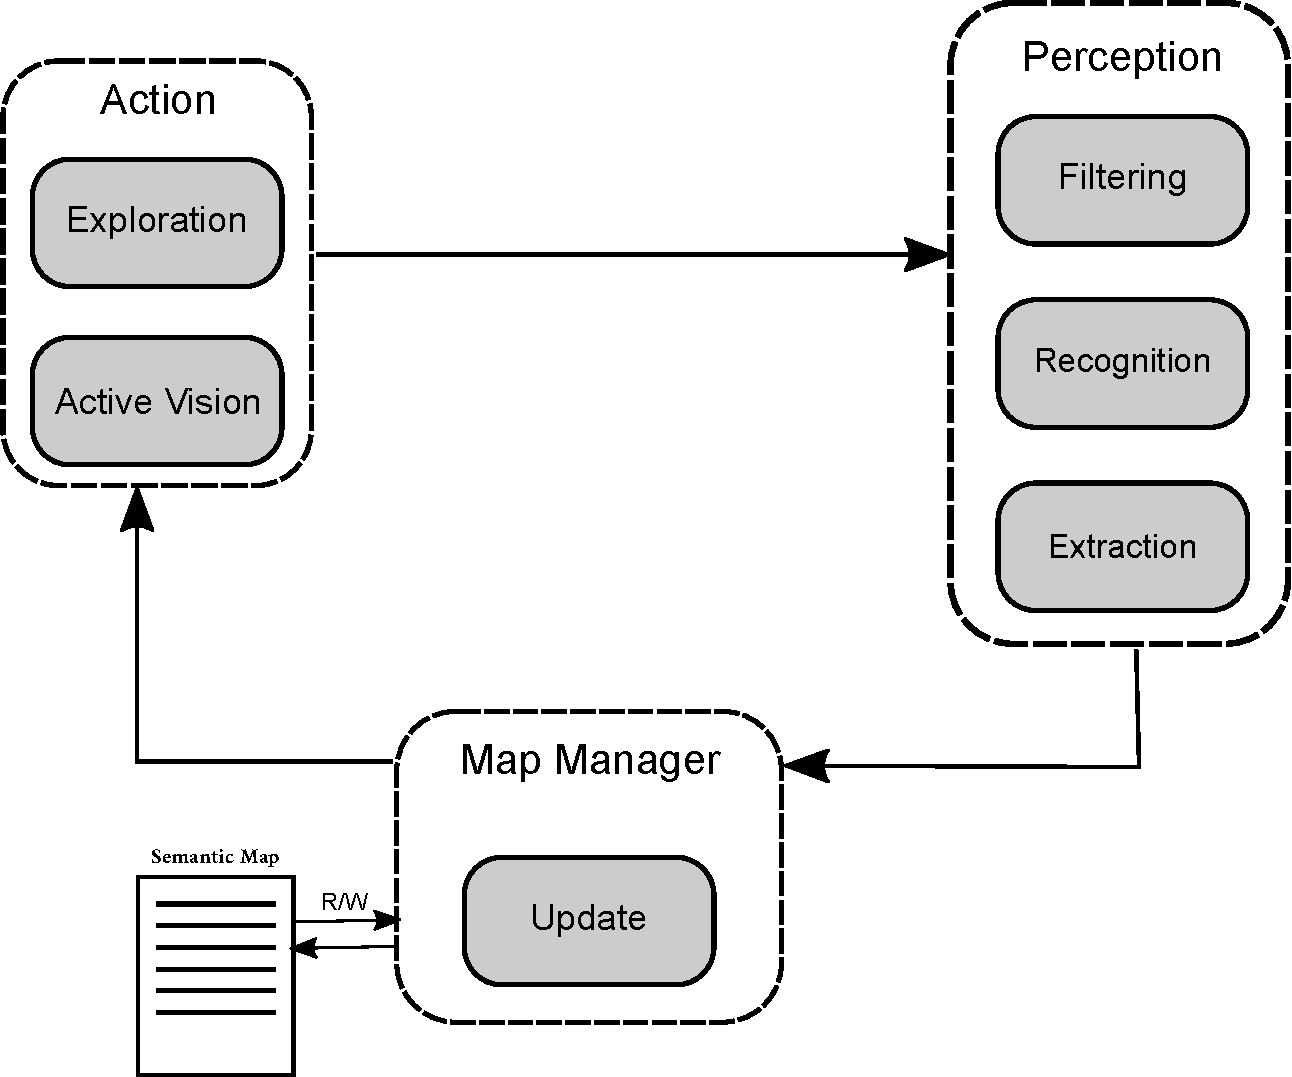
\includegraphics[width=\linewidth]{pics/drawing-crop.pdf}
		\caption{Semantic mapping system.}
		\label{fig:system}
	\end{figure}
		
	\section{Perception}
	
%	The perception module takes every frame coming from the RGB-D camera and has to tell which objects are seen by the robot. 
%	

	\begin{itemize}
		\item The perception module takes as input sensor measurements $\cS = \{ \bs_1 \dots \bs_T \}$ acquired by the robot during exploration and returns a list of elements $\cE = \{ \bE_1 \dots \bE_N \}$
		
		\item This information is passed to the map manager to update the robot knowledge of the environment.
		
		\item 	Possible approaches are:
		\begin{itemize}
			\item {\bf Geometric only:} consists in recovering only the geometric structure of the environment.
			\item {\bf Semantic only:} focuses on the extraction of semantic information from sensory data, assuming that no reconstruction is needed.
			\item {\bf Pipelined:} consists in recovering a geometric model of the environment and, subsequently, using this model to extract semantic information.
			\item {\bf Parallel:} reconstruction and recognition are performed separately (and simultaneously) and then, their results are fused together by the symbol grounding module.
			\item {\bf Joint:} in this approach, perception is formulated as a problem that jointly estimates geometric structure and semantic properties of the environment. 
		\end{itemize}
	\end{itemize}
	
	\subsection{Reconstruction}

	\begin{itemize}
		\item Consists in processing sensor measurements $\cS$ to recover both the set of robot poses $\cX = \{ \bx_1 \dots \bx_T \}$ and a digital representation of the environment $\cM$ (e.g., occupancy grid, point cloud, topological graph, etc...).
		\item 	In literature,  different types of representation have been proposed, as well as different methods to obtain each of them.
		\begin{itemize}
			\item {\bf Metric:} can be used to measure physical quantities in the environment such as distance to obstacles.
			\item {\bf Topological:} allows the robot to assess the connectivity between places and/or objects in the environment.
		\end{itemize}
	\end{itemize}	
		
	\subsection{Recognition}
	
%	Extracting semantic information from visual data is one of the  fundamental problems of computer vision. Recognition can be decomposed into sub-tasks, depending on the information one is interested to extract from the input data. These sub-tasks can be organized on a progression that goes from coarse to fine grained inference. 
%	
	\begin{itemize}
		\item Consists in extracting subsets of sensory data (patterns) belonging to known objects and scenes categories and assign them the corresponding semantic label.
		\item In robotic applications, input data can be of two types:
		\begin{itemize}
			\item {\bf Raw}: recognition is performed directly on sensor data and each time the sensor returns a measurement.
			\item {\bf Reconstructed}: recognition is performed on a scene obtained with reconstruction methods.
		\end{itemize}
		\item The output of the recognition step consists in a list of detections $\cD = \{ \bd_1 \dots \bd_N \}$, that, in general, may contain just one element (classification) or a sequence of them (detection, segmentation). Each entry in the detection list $\bd_i$ is characterized by: 
		\begin{itemize}
			\item {\bf Semantic Label}: $l \in \cL$ that identifies the semantic category of the detection. 
			\item {\bf Spatial Location}: that express the position of the detection w.r.t. the reference system of the input data.
		\end{itemize}
		\item 	Possible approaches are:
		\begin{itemize}
			\item {\bf Image classification:} assigning a semantic label to an input image from a fixed set of categories.
			\item {\bf Object detection:} making a prediction not only of object categories but also of their spatial locations.
			\item {\bf Image segmentation:} finding groups of pixels that possess some "similarity" among each other.
			\item {\bf Scene labeling:} assigning a semantic label to each geometric feature of the scene.
			\item {\bf 3d object recognition:} given an input model and a models database, finds the model in the database that best matches with the input.
			\item {\bf 3d object detection:} given an input model and a 3d scene, finds the location of the input model inside the scene.
		\end{itemize}
	\end{itemize}

	\section{Map Management}
	
	\begin{itemize}
		\item The map manager has the task of incrementally updating the semantic map with new information coming from the perception module. 
		\item The update can be performed:
		\begin{itemize}
			\item {\bf Off-line:} the semantic map is built after all sensor measurements have been acquired by the robot during exploration.
			\item {\bf Frame-by-frame:} the map is built while the robot is exploring the environment and acquiring sensor measurements.
			\item {\bf Without KB:} the semantic map contains only the list of elements.
			\item {\bf With KB:} the elements in the semantic map are linked to predicates in a KB.
		\end{itemize}
		\item In order to renew the semantic map each time a new sensor measurement is acquired, it's necessary to maintain a correspondence between the objects being observed and their internal representations.
		\item The input to the map management module is the list of elements $\cSM^R$ returned by the perception module, where the superscript $R$ denotes that the elements are expressed in the robot local reference frame.
		\item After matching the elements in $\cSM^R$ with those already seen and contained in $\cSM^G$, where the superscript $G$ denotes that the elements are expressed in the global reference frame, the incoming information is inserted in the semantic map, in order to return an up to date version of $\cSM^R$.
	\end{itemize}
	
	\subsection{Matching}
	
	\begin{itemize}
		\item Consists in finding the set of correspondences $\cC = \{\bc_1 \dots \bc_K\}$ between elements in the robot local map $\cSM^R$ and elements in the global map $\cSM^G$.
		\item A correspondence between two elements can be assessed through a similarity measure $d(\bE_i^R,\bE_j^G)$.
		\item The $k$-th correspondence $\bc^{i,j}_k \eq <\bE_i^R,\bE_j^G>$ establishes that the $j^{th}$ element $\bE_j^G$ in the global map is the "closest" to the $i^{th}$ element $\bE_i^R$ in the local map . That is:
		\begin{equation}
			\bE_i^R = \argmin_{\bE_i} \, d(\bE_i^R,\bE_j^G)
		\end{equation} 
		\item Possible approaches are:
		\begin{itemize}
			\item $\dots$
		\end{itemize}
	\end{itemize}
	
	\subsection{Update}
	
	\begin{itemize}
		\item Consists in inserting new information coming from sensor measurements in the environment representation of the robot.
		\item The result of this processing step is an updated map.
		\item It receives as input the set of correspondences $\cC$. Then, for each correspondence $\bc^{i,j}_k$ it's possible to perform two operations:
		\begin{itemize}
			\item $d(\bE_i^R,\bE_j^G) \leq d_{th}$: $\bE_i^R$ matches with $\bE_j^G$ $\rightarrow$ Merge the two elements.
			\item $d(\bE_i^R,\bE_j^G) > d_{th}$: $\bE_i^R$ has not been already seen $\rightarrow$ Add the element to the map.
		\end{itemize}
		\item Possible approaches are:
		\begin{itemize}
			\item {\bf Bayesian:} the update of an element considers past observations.
			\item {\bf Context aware:} the update of an element considers also spatial relations with other elements.
		\end{itemize}
	\end{itemize}
	
	\subsection{Symbol Grounding}
	
	\begin{itemize}
		\item Consists of linking symbols, the elements in $\cSM^G$, to concepts in a Knowledge Base (KB).
		\item Possible approaches are:
		\begin{itemize}
			\item $\dots$
		\end{itemize}
	\end{itemize}	

	\section{Action}
	
	The action module has the task of navigating the robot in a way to improve its current knowledge of the environment. To do so, it receives the current belief of the problem state, i.e. map and robot pose, and plans a motion trajectory that maximizes some cost function based on different criteria, e.g., navigation cost, information cost, and so on.
	
	\clearpage
	
	\documentclass{article}

\usepackage{graphicx}
\usepackage{amsmath}
\usepackage{amsfonts}
\usepackage{multirow}

%% Key definitions for text elements. USE THEM
\def\secref#1{Sec.~\ref{#1}}
\def\figref#1{Fig.~\ref{#1}}
\def\tabref#1{Tab.~\ref{#1}}
\def\eqref#1{Eq.~(\ref{#1})}
\def\algref#1{Alg.~\ref{#1}}
\def\appref#1{App.~\ref{#1}}

\newcommand\etal{\emph{et al.}}

%\usepackage{amsopn}


\newcommand{\bJidx}[1]{\ensuremath{\mathbf{J}^{[#1]}}}
\newcommand{\cose}{\mathrm{cose}}
\newcommand{\bzidx}[1]{\mathbf{z}^{[{#1}]}}
\newcommand{\bxidx}[1]{\mathbf{x}^{[{#1}]}}
\newcommand{\bhidx}[1]{\mathbf{h}^{[{#1}]}}
\newcommand{\bOmegaidx}[1]{\mathbf{\Omega}^{[{#1}]}}
\newcommand{\bSigmaidx}[1]{\mathbf{\Sigma}^{[{#1}]}}
\newcommand{\bHidx}[1]{\mathbf{H}^{[{#1}]}}

\newcommand{\bv}{\mathbf{v}}
\newcommand{\bl}{\mathbf{l}}
\newcommand{\bt}{\mathbf{t}}
\newcommand{\bo}{\mathbf{o}}
\newcommand{\bM}{\mathbf{M}}
\newcommand{\bL}{\mathbf{L}}
\newcommand{\bA}{\mathbf{A}}
\newcommand{\bB}{\mathbf{B}}
\newcommand{\bE}{\mathbf{E}}
\newcommand{\bK}{\mathbf{K}}
\newcommand{\bC}{\mathbf{C}}
\newcommand{\bH}{\mathbf{H}}
\newcommand{\bI}{\mathbf{I}}
\newcommand{\bP}{\mathbf{P}}
\newcommand{\bX}{\mathbf{X}}
\newcommand{\bZ}{\mathbf{Z}}
\newcommand{\bR}{\mathbf{R}}
\newcommand{\bS}{\mathbf{S}}
\newcommand{\bU}{\mathbf{U}}
\newcommand{\bV}{\mathbf{V}}
\newcommand{\bT}{\mathbf{T}}
\newcommand{\bpi}{\mathbf{\pi}}
\newcommand{\btl}{\mathbf{tl}}
\newcommand{\bbr}{\mathbf{br}}


\newcommand{\iD}{\mathbf{D}}
\newcommand{\iN}{\mathbf{N}}
\newcommand{\iI}{\mathbf{I}}

\newcommand\norm[1]{\left\lVert#1\right\rVert}

\newcommand{\bzridx}[1]{\ensuremath{\mathbf{z}^{({#1})}}}
\newcommand{\bxridx}[1]{\mathbf{x}^{({#1})}}
\newcommand{\bhridx}[1]{\mathbf{h}^{({#1})}}

\newcommand{\bJ}{\mathbf{J}}
\newcommand{\bZero}{\mathbf{0}}

\newcommand{\cS}{\mathcal{S}}
\newcommand{\cE}{\mathcal{E}}
\newcommand{\cC}{\mathcal{C}}
\newcommand{\cSM}{\mathcal{SM}}
\newcommand{\cR}{\mathcal{R}}
\newcommand{\cM}{\mathcal{M}}
\newcommand{\cP}{\mathcal{P}}
\newcommand{\cL}{\mathcal{L}}
\newcommand{\cD}{\mathcal{D}}
\newcommand{\cZ}{\mathcal{Z}}
\newcommand{\cX}{\mathcal{X}}
\newcommand{\range}[3]{#1_{#2:#3}}


\newcommand{\ba}{\mathbf{a}}
\newcommand{\bb}{\mathbf{b}}
\newcommand{\bc}{\mathbf{c}}
\newcommand{\bd}{\mathbf{d}}
\newcommand{\be}{\mathbf{e}}
\newcommand{\ec}{\mathbf{e}}
\newcommand{\bm}{\mathbf{m}}
\newcommand{\bg}{\mathbf{g}}
\newcommand{\Dim}{\mathrm{Dim}}

\newcommand{\bs}{\mathbf{s}}
\newcommand{\bx}{\mathbf{x}}
\newcommand{\by}{\mathbf{y}}
\newcommand{\br}{\mathbf{r}}
\newcommand{\bz}{\mathbf{z}}
\newcommand{\bu}{\mathbf{u}}
\newcommand{\bn}{\mathbf{n}}
\newcommand{\bh}{\mathbf{h}}
\newcommand{\bff}{\mathbf{f}}
\newcommand{\bp}{\mathbf{p}}
\newcommand{\bDelta}{\mathbf{\Delta}}
\newcommand{\bGamma}{\mathbf{\Gamma}}
\newcommand{\bDeltaalpha}{\mathbf{\Delta \alpha}}
\newcommand{\bDeltar}{\mathbf{\Delta r}}
\newcommand{\bDeltax}{\mathbf{\Delta x}}
\newcommand{\bDeltaX}{\mathbf{\Delta X}}
\newcommand{\bDeltat}{\mathbf{\Delta t}}
\newcommand{\bDeltaR}{\mathbf{\Delta R}}
\newcommand{\tTov}{\mathrm{t2v}}
\newcommand{\vTot}{\mathrm{v2t}}

\newcommand{\bO}{\mathbf{O}}

\newcommand{\defeq}{=}


\newcommand{\bmu}{\mathbf{\mu}}
\newcommand{\bnu}{\mathbf{\nu}}
\newcommand{\bSigma}{\mathbf{\Sigma}}
\newcommand{\bOmega}{\mathbf{\Omega}}
\newcommand{\bLambda}{\mathbf{\Lambda}}

\newcommand{\mat}[1]{#1}
\newcommand{\mbf}[1]{\mathbf{#1}}
\newcommand{\defn}[1]{\emph{#1}}

\newcommand{\mysum}{\sum}
\newcommand{\myprod}{\prod}
\newcommand{\eq}{=}
\newcommand{\pv}{\mathrm{P}}
%\newcommand{\implies}{\Rightarrow}
\newcommand{\Parents}{\mathrm{Parents}}
\newcommand{\rj}{\mathrm{j}}
\newcommand{\proj}{\mathrm{proj}}
\DeclareMathOperator*{\argmax}{argmax}
\DeclareMathOperator*{\argmin}{argmin}
\DeclareMathOperator*{\atantwo}{atantwo}

\newcommand{\mR}{\mathbb{R}}
\newcommand{\mN}{\mathbb{N}}
\newcommand{\mC}{\mathbb{C}}



\begin{document}
			
	\begin{table}
		%\centering
		\begin{tabular}{|c|c|c|c|c|c|c|c|}
			\hline
			 & Matching & Update & Exploration & Active Vision & Filtering & Recognition & Extraction \\
			\hline
			\cite{ulrich2000icra} &  &  &  &  &  & x &  \\ 
			\hline 			 
			\cite{swain1991ijcv} &  &  &  &  &  & x &  \\ 
			\hline 			 
			\cite{torralba2003context} &  &  &  &  &  & x &  \\ 
			\hline 			 
			\cite{oliva2001ijcv} &  &  &  &  &  & x &  \\ 
			\hline 			 
			\cite{lisin2005cvpr} &  &  &  &  &  & x &  \\ 
			\hline 			 
			\cite{viola2004ijcv} &  &  &  &  &  & x &  \\ 
			\hline 			 
			\cite{papageorgiou1998iccv} &  &  &  &  &  & x &  \\ 
			\hline 			 
			\cite{freund1997jcss} &  &  &  &  &  & x &  \\ 
			\hline 			 
			\cite{dalal2005cvpr} &  &  &  &  &  & x &  \\ 
			\hline 			 
			\cite{krizhevsky2012nipsjournal} &  &  &  &  &  & x &  \\ 
			\hline 			 
			\cite{redmon2016cvpr,erhan2014cvpr,liu2016eccv} &  &  &  &  &  & x &  \\ 
			\hline 			 
			\cite{long2015cvpr} &  &  &  &  &  & x &  \\ 
			\hline 			 
			\cite{simonyan2014very,szegedy2015cvpr} &  &  &  &  &  & x &  \\ 
			\hline 			 
			\cite{de2017cvpr} & x & x &  &  &  & x &  \\ 
			\hline 			 
			\cite{stuckler2012iros} & x & x &  &  &  & x &  \\ 
			\hline 			 
			\cite{herbst2014icra} & x & x &  &  &  & x &  \\ 
			\hline 			 
			\cite{vineet2015icra} & x & x &  &  &  & x &  \\ 
			\hline 			 
			\cite{zender2008ras} & x & x &  &  &  & x &  \\ 
			\hline 			 
			\cite{nuchter2008ras} & x & x &  &  &  & x &  \\ 
			\hline 			 
			\cite{xiong2010bmvc} & x & x &  &  &  & x &  \\ 
			\hline 			 
			\cite{blaha2016cvpr} & x & x &  &  &  & x &  \\ 
			\hline 			 
			\cite{kundu2014eccv} & x & x &  &  &  & x &  \\ 
			\hline 			 
			\cite{sengupta2013icra} & x & x &  &  &  & x &  \\ 
			\hline 			 
			\cite{hane2013cvpr} & x & x &  &  &  & x &  \\ 
			\hline 			 
			\cite{yamauchi1997cira,yamauchi1998frontier,wang2011frontier} &  &  & x &  &  &  &  \\ 
			\hline 			 
			\cite{senarathne2013efficient,keidar2012robot} &  &  & x &  &  &  &  \\ 
			\hline 			 
			\cite{oriolo2004icra,freda2005icra} &  &  & x &  &  &  &  \\ 
			\hline 			 
			\cite{lavalle1998rapidly} &  &  & x &  &  &  &  \\ 
			\hline 			 
			\cite{bircher2016icra} & & & x &  &  &  &  \\ 
			\hline 			 
			\cite{el2013improved,franchi2009sensor} &  &  & x &  &  &  &  \\ 
			\hline 			 
		\end{tabular}
		\caption{Data association.}
		\label{tab:assoc}
	\end{table}
	
	\clearpage
	\bibliography{references}
	\bibliographystyle{plain}
	
\end{document}
	
	\clearpage

	\section{Our Approach}
	
	A semantic map is a triple:
	
	\begin{equation}
	\cSM = < \cR, \cM, \cP >,
	\end{equation}
	
	\noindent
	with:
		
	\begin{description}
		\item {\bf Global Reference System} $\cR$: the reference system is used to express all the elements of the map in a single frame.
		\item {\bf Metric Map} $\cM$: the metric information $\cM$ of the semantic map can be seen as a collection of 3D geometric models:
		
		\begin{equation}
		\cM = \{\bM_1 \cdots \bM_N\},
		\end{equation}
		
		\noindent	
		where each model $\bM_i$ is an entity defined by:
		
		\begin{itemize}
			\item {\bf Pose3D}: $\bX = [ \bR | \bt] \in SE(3)$,
			\item {\bf Size3D}: $\bS = <\bL ,\bU> \in \mathbf{R}^3 $,
			\item {\bf Representation3D}: e.g. a point cloud, a mesh and so on.
		\end{itemize}
		
		The adopted convention is that the pose $\bX$ is assumed to refer to the centroid of the model and that the bounding box $\bS$ is defined by two 3D vectors that specify its "lower" and "upper" corners.
		\item {\bf Property Map} $\cP$: the semantic information $\cP$ contains the assertions about the properties of the objects in $\cM$:
		
		\begin{equation}
		\cP = \{\bP_1 \cdots \bP_N\},
		\end{equation}
		
		\noindent
		where each $\bP_i$ is a set of predicates of $arity = (1 \dots q)$ that are instances of $\bm_i$ (corresponding to the geometrical object $\bM_i$).
	\end{description}	

	\noindent
	Possible operations on the map are:
	
	\begin{itemize}
		\item query for object: given an object it's possible to check if it's already present in the map
		\item update object: allows to update an object present in the map with a new observation
		\item add object: allows to add an object to the map if it's seen for the first time
		\item render map: builds a 3d model from the collection of objects, this function can be used for navigation and visualization.
		\item serialize/deserialize: these functions allow to save a map on disk and to load it for later use.
	\end{itemize}
			
	\subsection{Perception}

	Some preliminary notation:
	
	\begin{itemize}
		\item {\bf Image domain}: $\bOmega = \{(u,v) \in \mN^2 \mid u \in [0,height], v \in [0,width]\}$
		\item {\bf RGB domain}: $\bGamma = \{(r,g,b) \in \mN^3 \mid r \in [0,255], g \in [0,255], b \in [0,255]\}$
		\item {\bf Depth domain}: $\bDelta = \{ d \in \mR \mid d \in [0,1]\}$
		\item {\bf Label domain}: $\bLambda = \{ l \in \mN \mid l \in [0,N]\}$
		\item {\bf Pixel}: $\bx \in \bOmega$
		\item {\bf RGB image}: $I : \bOmega \rightarrow \bGamma \implies \bx \rightarrow I(\bx)$
		\item {\bf Depth image}: $D : \bOmega \rightarrow \bDelta \implies \bx \rightarrow D(\bx)$
		\item {\bf Label image}: $L : \bOmega \rightarrow \bLambda \implies \bx \rightarrow L(\bx)$
	\end{itemize}
	
	\noindent
	{\bf Recognition:} 
	finding instances of known class objects in the input image. More formally, given an RGB image $I$ and a set of semantic labels $\cL = \{ l_1 \dots l_N \}$, computes an assignment $L(\bx)$ of labels $l_i$ to each image pixel $\bx$.
	
	\noindent
	{\bf Input: }
	\begin{itemize}
		\item {\bf RGB Image}: $I$
		\item {\bf Semantic Labels}: $\cL$
	\end{itemize}
	\noindent
	{\bf Output: }
	\begin{itemize}
		\item {\bf Label Image}: $L$
	\end{itemize}
	
	\noindent
	{\bf Reconstruction:} 
	given an initial guess $\cX_0$ regarding a set of variables $\cX = \{\bx_1 \dots \bx_n\}$ (which includes robot trajectory and landmark positions) and a set of sensor measurements $\cZ = \{\bz_1 \dots \bz_m\}$, computes the assignment of variables $\cX^\star$ that maximizes the posterior $p(\cX \mid \cZ)$.
	
	\noindent
	{\bf Input: }
	\begin{itemize}
		\item {\bf Initial guess}: $\cX_0$
		\item {\bf Sensor Measurements}: $\cZ$
	\end{itemize}
	\noindent
	{\bf Output: }
	\begin{itemize}
		\item {\bf MAP estimate}: $\cX^\star$
	\end{itemize}
	
	\subsection{Mapping}
	
	Given the above definition of semantic map, let 
	
	\begin{equation}
	\bE_i \eq < \bM_i,\bP_i >
	\end{equation}
	
	\noindent
	denote the $i^{th}$ element of $\cSM$, where: $\bM_i \in \cM$ is the metric component (expressed in $\cR$) and $\bP_i \in \cP$ the semantic properties. 
	
	Depending on $\cR$, we consider two different maps. The global map $\cSM^G_t = < \cR^G, \cM^G, \cP^G >$  is the collection of elements $\{ \bE_1^G \dots \bE_N^G \}$ referred to the global reference frame at time $t$. While, the local map $\cSM^L_t = < \cR^L, \cM^L, \cP^L >$ is the collection of elements $\{ \bE_1^L \dots \bE_M^L \}$ referred to the robot reference frame at time $t$. 
	
	{\bf Symbol Grounding:}
	this module is in charge of updating the current belief of the robot about the state of the environment, expressed in $\cSM^G_t$, with the new information contained in $\cSM^L_t$. This is done by first finding the set of correspondences $\cC_t = \{\bc_1 \dots \bc_K\}$ that states which elements in the global map $\cM^G$ correspond to the one observed in the local map $\cM^L$. In particular, the $k$-th correspondence
	
	\begin{equation}
	\bc^{i,j}_k \eq <\bE_i^G,\bE_j^L> 
	\end{equation}
	
	\noindent
	establishes that the $j^{th}$ element $\bE_j^L$ in the local map is the "closest" (w.r.t. a similarity measure, see below) to the $i^{th}$ element $\bE_i^G$ in the global map. Thus, computing a correspondence $\bc^{i,j}_k$ consists in finding the element $\bE_j^\star$ that satisfies:
	
	\begin{equation}
	\bE_j^\star = \argmin_{\bE_j} \, d(\bE_i^G,\bE_j^L)
	\end{equation}
	
	
	
	Then, according to $d(\bE_i^G,\bE_j^L)$, it's possible to perform two operations to update of the map:
	
	 \begin{itemize}
	 	\item $d(\bE_i^G,\bE_j^L) \leq d_{th}$: $\bE_j^L$ matches with $\bE_i^G$ $\rightarrow$ Merge the two elements
	 	\item $d(\bE_i^G,\bE_j^L) > d_{th}$: $\bE_j^L$ has not been already seen $\rightarrow$ Add the element to the map
	 \end{itemize}
	
	
	\noindent
	{\bf Input: }
	\begin{itemize}
		\item {\bf Global Map}: $\cSM^G_t$
		\item {\bf Local Map}: $\cSM^L_t$
	\end{itemize}
	\noindent
	{\bf Output: }
	\begin{itemize}
		\item {\bf Correspondences}: $\cC_t$	
		\item {\bf Updated Global Map}: $\cM_{t+1}^G$	
	\end{itemize}
	

	\clearpage	
	\bibliography{references}
	\bibliographystyle{apalike}
	
\end{document}

%	\subsection{Global Reference System}	
%	
%	The reference system is used to express all the elements of the map in a single frame.
%	
%	\subsection{Metric Map}	
%	
%	The metric information $\cM$ of the semantic map can be seen as a collection of 3D geometric models:
%	
%	\begin{equation}
%	\cM = \{\bM_1 \cdots \bM_N\},
%	\end{equation}
%	
%	\noindent	
%	where each model $\bM_i$ is an entity defined by:
%	
%	\begin{itemize}
%		\item {\bf Pose3D}: $\bX = [ \bR | \bt] \in SE(3)$,
%		\item {\bf Size3D}: $\bS = <\bL ,\bU> \in \mathbf{R}^3 $,
%		\item {\bf Representation3D}: e.g. a point cloud, a mesh and so on.
%	\end{itemize}
%	
%	The adopted convention is that the pose $\bX$ is assumed to refer to the centroid of the model and that the bounding box $\bS$ is defined by two 3D vectors that specify its "lower" and "upper" corners.
%	
%	\subsection{Property Map}	
%	
%	The semantic information $\cP$ contains the assertions about the properties of the objects in $\cM$:
%	
%	\begin{equation}
%	\cP = \{\bP_1 \cdots \bP_N\},
%	\end{equation}
%	
%	\noindent
%	where each $\bP_i$ is a set of predicates of $arity = (1 \dots q)$ that are instances of $\bm_i$ (corresponding to the geometrical object $\bM_i$).